\section{Reduzindo a dimensionalidade de um problema}

\begin{frame}{Variância}
  \begin{figure}[t]
    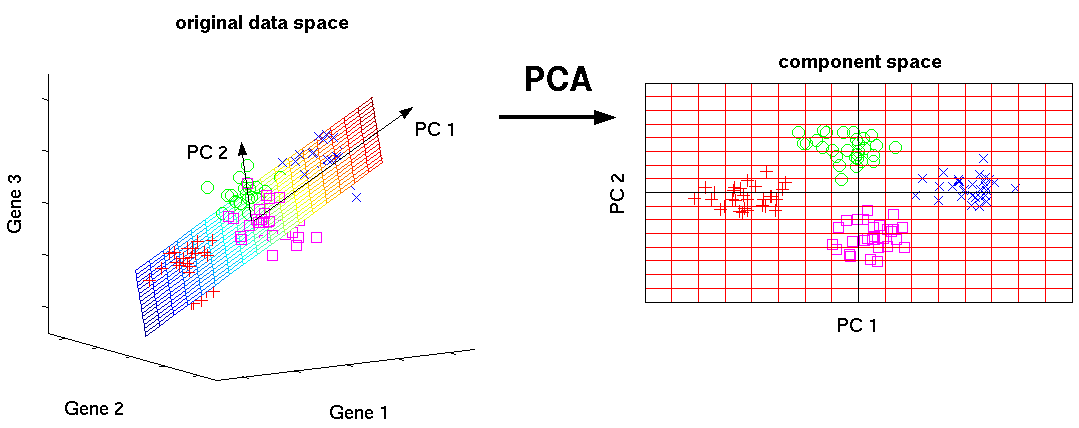
\includegraphics[width=\textwidth]{pca.png}
    \caption{Fonte: \cite{scholz2006approaches}}
    \centering
  \end{figure}
\end{frame}

\begin{frame}{Problema}

  \begin{table}
    \centering
    \begin{tabular}{ |c|c|c|c|c|c| }
    \hline
    & $x_1$ & $x_2$ & $\cdots$ & $x_{n-1}$ & $x_{n}$ \\ 
    \hline
    1 & & & & & \\ 
    \hline
    2 & & & & & \\ 
    \hline
    $\vdots$ & & & & & \\ 
    \hline
    m & & & & & \\ 
    \hline
    \end{tabular}
    \caption{Tabela com $n$ características e $m$ observações}
  \end{table}

  \begin{itemize}
    \item Como escolher os componentes (características) mais importantes?
  \end{itemize}

\end{frame}

\begin{frame}{Variância}
  \[ \sigma^2 = \frac{1}{n-1} \vt{x} \trans{\vt{x}} \]
  onde $n = \norm{\vt{x}}$.
\end{frame}

\begin{frame}{Covariância}
  \begin{defn}{Variáveis aleatórias em vetores coluna:}
    \[ \cov{x}{y} = \exptd{(\vt{x} - \exptd{\vt{x}}) \trans{(\vt{y} - \exptd{\vt{y}})}} \]

    \begin{align*}
      \cov{x}{x} &= \exptd{(\vt{x} - \exptd{\vt{x}}) \trans{(\vt{x} - \exptd{\vt{x}})}}\\
      &= \exptd{\vt{x} \trans{\vt{x}}}
    \end{align*}
  \end{defn}
\end{frame}

\begin{frame}{Covariância}

\end{frame}

